\documentclass[a4paper,USenglish]{socg-lipics-v2018}
\usepackage{amsthm}
\usepackage{amsmath}
\usepackage{mathbbol}
\usepackage{amsfonts}
\usepackage{amssymb}
\usepackage{graphicx}
\usepackage{algorithm}
\usepackage{url}
%\usepackage{floatflt}
%\usepackage{mathptmx}
\usepackage{epsfig}
\usepackage{wrapfig}
\usepackage{color}

\usepackage{algorithm}
\usepackage{algpseudocode}
\usepackage{comment}
\usepackage{braket}

% \usepackage{ccaption}

\newcommand{\N}{\mathbb{N}}
\newcommand{\Q}{\mathbb{Q}}
\newcommand{\R}{\mathbb{R}}
\newcommand{\Z}{\mathbb{Z}}
\renewcommand{\S}{\mathbb{S}}
\newcommand{\dappr}{\tilde{d}}
%\newcommand{\Wlog}{W.l.o.g.\ }
%\newcommand{\wlog}{w.l.o.g.\ }
\newcommand{\eps}{\epsilon}
\newcommand{\orient}{O}
\newcommand{\cpro}{\Pi}
\newcommand{\fib}{\mathrm{Fib}}

\newcommand{\parent}{\mathrm{par}}
\newcommand{\point}{p}
\newcommand{\level}{\ell}
\newcommand{\diam}{\mathrm{diam}}
\newcommand{\pointset}{P}
\newcommand{\distspace}{\mathcal{M}}
\newcommand{\dist}{\delta}
\newcommand{\adist}{\gamma}
\newcommand{\complexity}{C_{\dist}}
\newcommand{\doublingdimension}{\Delta}

%\newcommand{\remark}[1]{\textbf{[#1]}}

%\newtheorem{theorem}{Theorem}
%\newdef{definition}{Definition}
%\newtheorem{lemma}[theorem]{Lemma}
%\newtheorem{corollary}[theorem]{Corollary}

\newcommand{\myparagraph}[1]{\textbf{#1.}}

%\newtheorem{theorem}{Theorem}
%\newtheorem{lemma}[theorem]{Lemma}
%\newtheorem{proposition}[theorem]{Proposition}
%\newtheorem{corollary}[theorem]{Corollary}
%\newtheorem{definition}[theorem]{Definition}
%\newtheorem{remark}[theorem]{Remark}
%\newtheorem{note}[theorem]{Note}

%\numberwithin{equation}{section}
%\numberwithin{figure}{section}

%\def\marrow{\marginpar[\hfill$\longrightarrow$]{$\longleftarrow$}}
%\def\michael#1{\textcolor{red}{\textsc{Michael says: }{\marrow\sf #1}}}

\title{Geometric Filters for Metric Spaces}
\author{Michael Kerber}{TU Graz}{kerber@tugraz.at}{}{}
\author{Arnur Nigmetov}{TU Graz}{nigmetov@tugraz.at}{}{}

\begin{document}
\maketitle

\section{Introduction}

\paragraph{Motivation.}
%
Given a set $\pointset:=\{p_1,\ldots,p_n\}$ of $n$ points
in a metric space $(\distspace,\dist)$, 
consider the following standard operations:

\begin{description}
\item[Nearest Neighbor] Given a point $q\in\distspace$,
find $p_i\in\pointset$ such that, for all $j=1,\ldots,n$,
\[d(q,p_i)\leq d(q,p_j)\]

\item[Metric approximation] Given $\eps>0$, compute a metric $\adist$
such that for all $1\leq i,j\leq n$,
%
\[\dist(p_i,p_j)\leq \adist(p_i,p_j) \leq (1+\eps) \dist(p_i,p_j).\]

By ``computing'' $\adist$, we mean to compute a $n\times n$-matrix $E$ 
such that $E_{ij}=\adist(p_i,p_j)$.
\end{description}

Assume that an algorithm is given to compute $\dist(\cdot,\cdot)$
for any two points in $\distspace$ in worst-case complexity $\complexity$.
Then trivially, the above problems can be solved (exactly) in
$O(n\complexity)$ and $O(n^2\complexity)$ time, respectively.
For low-dimensional\footnote{we will make this notion precise
later in the text} metric spaces, we can improve these bounds:
Using cover trees~\cite{cover-trees}, we can preprocess the point set
in $O(\complexity n\log n)$ time to answer nearest neighbor queries
in $O(\complexity \log n)$ time. Combining cover trees with well-separated
pair decompositions (WSPD), we obtain an $\eps$-spanner for the graph
induced by $\dist$ in $O(\complexity n\log n)$ time and
of linear size (assuming, for simplicity, that $\eps$ is a constant).
Out of this spanner,
we can construct an approximate metric
with an all-pair shortest path computation,
resulting in a total running time of
\[O(\complexity n\log n+ n^2\log n)\]
using Johnson's algorithm~\cite{johnson}.

In the aforementioned techniques, $\complexity$ is usually considered
as a constant-time operation and hence ignored in the analysis.
There are good reasons for that: the most common case of a metric space
is $\distspace=\R^d$ with $d$ some constant, in which case $\dist$ can be evaluated in $O(d)=O(1)$ time.
Even if $d$ is considered non-constant,
it can always be assumed that $d\leq n$, hence $\complexity$ is at most $O(n)$.
Another typical assumption is that all pairwise distances are part of the input
in which case $\complexity$ is $O(1)$.

However, we argue that in some situations, distance computations
in $\distspace$ can be costly and $\complexity$ might be incomparable
with $n$. Our motivating examples come from topological summaries
such as persistence diagrams or Reeb graphs, which are of interest
in the field of topological data analysis. A persistence diagram
is a point set in $\R^2$, and the distance between two diagrams
is determined by a min-cost matching between the point sets.
If the diagrams have $N$ points, computing this matching requires
polynomial time in $N$, and $N$ might well be larger than $n$, the number
of diagrams considered. For the case of Reeb graphs, the situation is even
worse: while several metrics on Reeb graphs have been proposed,
not even an constant-factor approximation algorithm is known that runs
in polynomial time in the size of the graphs.

In the light of the above examples, we pose the question: 
how can we practically reduce the number of distance computations 
in algorithms for metric spaces?
Note that for low-dimensional spaces, the aforementioned techniques
already provide a partial solution: for approximating the metric, for instance,
we only compute $O(n\log n)$ distances instead of $O(n^2)$.


\paragraph{Contribution.}
%
We demonstrate that the number of distance computations can be further
reduced by a careful re-implementation of the underlying geometric algorithms.
Our improvement is based on the following simple observation: many geometric
constructions (such as cover tree and WSPD constructions) require distance
computations only in the form of the following predicate: 
``Is $\dist(p_i,p_j)\leq t$'', where $t$ is a real value.
We show that using the information of the already computed distances and
the triangle inequality, we can answer the above predicate in many cases
without computing the actual distance.

We describe our idea with an example. In Figure~\ref{fig:1st_example},
we see a weighted graph on $P$ whose edges are the distances that have
been computed so far; note that $\dist(p_1,p_2)$ is unknown. 
The shortest path from $p_1$ to $p_2$ has length $9$, which clearly
constitutes an upper bound on the distance by triangle inequality.
However, we can also infer that $\dist(p_1,p_2)\geq 3$:
otherwise, the path from $p_3$ to $p_4$ via $p_1$ and $p_2$
would be shorter than the edge $(p_3,p_4)$, again contradicting
triangle inequality.
Hence, the question whether $\dist(p_1,p_2)\leq t$ can be answered positively
for $t>=9$ and negatively for $t<3$. Only if $t\in[3,9)$, the actual
distance computation is necessary. This approach is reminiscent to the usage
of \emph{numerical filters} in geometric computing in the CGAL library,
where geometric predicates in exact number types are first evaluated using 
certified floating-point arithmetic, and exact computation is only
invoked if the numerical evaluation did not arrive at a decisive result
(e.g.~\cite{bbp-interval,kerber-phd}).

\begin{figure}[h]

\centering
\includegraphics[width=6cm]{intro_example.eps}
\caption{An example of a partially revealed metric.}
\label{fig:1st_example}
\end{figure}

In our implementation, we maintain the best lower and upper bounds of all
pairwise distances in an $n\times n$ matrix of intervals. We show how to
update this matrix in $O(n^4)$ time when a new edge is added.
%We point out once more that a quadratic update time only pays off
%if distance computations are expensive, say $\complexity=\Omega(n^2)$.

We perform an extensive experimental evaluation of our idea.
We mostly concentrate on point clouds in Euclidean space~--
of course, the approach does not yield any performance benefits in that
situation because distance computations are cheap; however, the Euclidean
case provides a simple setup for experiments.
We investigate how the dimensionality, the clustering density, 
the approximation quality, and noise 
in the point cloud affect the number of distance computations.
Our result show that $\ldots$

We also provide some experimental results for the case of persistence diagrams
which motivated this line of research. We point out that the space of
persistence diagrams fails to be ``low-dimensional''. To be precise,
its doubling dimension is $\infty$, and a finite set of $n$ diagram
can have the worst-case doublng dimension $\log n$. This worst-case
behavior is also the expected one if the diagrams are chosen randomly
(in a sense made precise in Section~\ref{sec:metric_spaces_top_summaries}). 
However, we demonstrate that
for natural collections of persistence diagrams, a substantial fraction
of distance computations can be avoided. In detail, $\ldots$

%We also have derived two minor technical results necessary for 
%our implementation. First of all, since our underlying distance computation
%algorithm for persistence diagrams only returns approximate answers,
%we had to adapt all algorithms to cope with approximate distances.
%Moreover, we show how a WSPDs can be constructed
%out of cover trees (we only found 
%the theoretically more efficient version of
%net trees used in the literature, but net trees are more difficult to implement
%efficiently). Both results can be obtained using standard methods, 
%but seem to be not present in prior work.


\section{Notation and Preliminary Notions}



A metric space is called \textit{doubling} with \textit{doubling constant} $k$,
if every ball of radius $r$ can be covered by at most $k$ balls of radius $r/2$,
and $k$ is the smallest number having that property.
\textit{Doubling dimension} of a doubling space is defined as $\log k$
(since we usually ignore multiplicative constants, the base of the logarithm is not really important; however,
we always use $\log$ to denote the logarithm with base 2).
It is easy to see that a subspace of a space with doubling dimension $d$ 
is always doubling and has the doubling dimension $O(d)$ (but not necessarily $d$).


In this paper we consider some fixed metric space $(X, \dist)$, and, to get interesting
results we must assume doubling property.

We shall need the following lemma.

\begin{lemma}
\label{lem:packing_lemma_dd}
Let $(X,\dist)$ be a metric space of doubling dimension $d$, and let $P$ be a subset of a ball $B(x,R)$ in $X$ such that the distance between any two distinct points of $P$ is at least $r$.
Then $P$ is finite and cardinality of $P$ satisfies the inequality $|P| < 2^{md}$, where $m = 1 + \lceil \log (R/r) \rceil $. 
\end{lemma}

\begin{proof}
We can cover $B(x,R)$ with $2^d$ ball of radius $R/2$, each of these balls we can cover with $2^d$
balls of radius $R/4$, etc. Repeating this process $\lceil \log \frac{R}{r/2} \rceil = m $ times, 
we cover
$B(x, R)$ with $2^{md}$ balls of radius at most $r/2$. Since a ball of radius $r/2$ can contain at most one point from $P$, the claim follows.
\end{proof}


\section{Metric Approximation}

It is known that asymptotically optimal spanner can be constructed by the following greedy algorithm: 
start with an empty graph on vertices $p_i$,
sort all edges $\{p_i, p_j\}$ by the length $\dist(p_i, p_j)$ in ascending order and keep adding them to the graph
until it becomes a $1+\eps$-spanner. In our setting this is the most expensive approach, because it requires
computing all pairwise distances first.
the true distance belongs.


 In our setting this is the most expensive approach, because it requires
 computing all pairwise distances first. We propose an alternative approach (or rather a family of algorithms), which we call
 \textit{blind} spanner, meaning that the algorithm that builds a spanner does not have access to $\dist(p_i, p_j)$
 before it decides to add the edge $(p_i, p_j)$.
 The algorithm also maintains lower and upper bounds
 for all pairwise distances, which are updated after a new edge is added. and the stopping criterion
 is based on these bounds, namely, if $a_{i, j}$ and $b_{i,j}$ denote lower and upper bounds
 for the distance between $p_i$ and $p_j$, respectively, then the algorithm stops, if $b_{i,j} / a_{i, j} \leq 1 + \eps$
 for all $i \neq j$.

\begin{algorithmic}
\label{alg:blind_spanner}
\Function{BlindSpanner}{$P, \eps$}
    \State {$E \gets \emptyset$}
    \State {$a_{i,j} \gets 0$ for all $1 \leq i,j \leq n$}
    \State {$b_{i,j} \gets \infty$ for all $1 \leq i,j \leq n, i \neq j$}
    \While {$\exists i \neq j : b_{i,j} / a_{i,j} > 1 + \eps$}
    \State {$(i,j) \gets GetEdgeToAdd$}
    \State {$v \gets \dist(p_i, pj)$}
    \State {Add weighted edge $(p_i, p_j, v)$ to $E$}
    \State {$UpdateBounds(i, j, v)$}
    \EndWhile
\EndFunction
\end{algorithmic}


In this pseudocode we adopt the convention that a positive number divided by 0 is $\infty$
and $\infty$ is larger than any real number,
thus making the predicate in the while loop well-defined.  The procedure $UpdateBounds$ is desribed in the next subsection,
now we only mention that it updates all upper and lower bounds based on triangle inequality involving the edge $(p_i, p_j)$,
and the update is monotonic: no upper bound can increase, no lower bound can decrease, and, after the distance
between $p_i$ and $p_j$ is calculated, both $a_{i,j}$ and  $b_{i,j}$ are set to be $\dist(p_i, p_j)$.
The most important part of this algorithm is the way of choosing the next edge to be added, and
there are several possibilities, which give very different results.



The first possibility will be called \textsc{BlindGreedy}, where we choose a pair $(p_i, p_j)$ that maximizes
the ratio $b_{i,j} / a_{i,j}$. If the number of maximizing pairs is more than 1, we choose one of them at random.
Note that our conventions imply that in \textsc{BlindGreedy} the edges that have $a_{i,j} = 0$ or $b_{i,j} = \infty$
have the highest priority, so the algorithm first ensures that the graph is connected and there are positive
lower bounds for every edge before it will start adding any other edges.



The second possibility will be referred to as \textsc{BlindRandom}, where among all edges $(p_i, p_j)$
for which $b_{i,j} / a_{i,j} > 1 + \eps$ we choose one uniformly at random. We may vary this approach
by insisting that we must first create a connected graph, or that we must first have some positive lower bound
for all edges, and only after these requirements are satisfied, we consider other pairs.


The next option is to make an additional assumption: while
computing $\dist(\cdot, \cdot)$ exactly is costly, we have access to a cheap approximation algorithm
that gives, say, a $2$-approximation of $\dist$ much faster (the output of this approximation algorithm is guaranteed to
lie in $[\dist(p,q), 2 \dist(p,q)]$). In order to simplify notation, we now assume
that all pairwise distances between our points belong to $[1, 2^t]$ for some $t$.
We now introduce \textit{buckets} of the form $[2^k, 2^{k+2}]$ for $k = 0 \dots t$;
these intervals are not disjoint, but, by calling our algorithm we can assign
each pair $(p_i, p_j)$ to one of the buckets.
Indeed, let $v$ be the output of the approximation algorithm for $\dist(p,q)$,
then we know that the true distance is in $[v/2, v]$. We want to put the pair $(p,q)$ into the bucket
that fully contains this interval, thus we need to find $k$ such that
$2^k \leq v /2$ and $v \leq 2^{k+2}$. These inequalities give $ 2^{k+1} \leq v \leq 2^{k+2}$,
and we take $k = \lfloor \log v \rfloor - 1$.
If we find a bucket for each pair $(p_i, p_j)$, we have some sort of a weak ordering: we cannot say anything
about two edges that are assigned to the same bucket or to overlapping buckets, but if the buckets
are disjoint, we know which edge is longer. Now we can either imitate the greedy spanner (non-blind) algorithm,
traversing buckets in the order of their left endpoint, and adding edges from them; or we could alternate: in even iterations
we travers the buckets from left to right, adding edges from each bucket one by one, and in odd iterations
we traverse the buckets from right to left. This alternative makes sense, because we need to have good lower bounds in
order to build a blind spanner, and good lower bounds can be obtained from the triangle inequality, if one of the edges 
in a path connecting $p_i$ and $p_j$ in $G$ is longer than the sum of the lengths of all other edges.
We refer to the former option as \textsc{BlindQuasiSortedGreedy} and to the latter one as \textsc{BlindQuasiSortedShaker}.


 \paragraph{Maintaining Lower and Upper Bounds}

 In this subsection we explain the update procedure that we use. Suppose that
 $a_{k,l}$ and $b_{k,l}$ are valid lower and upper bounds, so that
\[
     \forall 1 \leq k < l \leq n \quad a_{k,l} \leq \dist(p_k, p_l) \leq b_{k,l}.
\]
Assume that $\dist(p_i,p_j)=v\in\R$ has been computed.
First, we reset $a_{i,j}$ and $b_{j,i}$ to $v$. 
To update the upper bound of some entry $b_{k,\ell}$,
we observe that the shortest path from $p_k$ to $p_\ell$ might now
go through the new edge. Hence, we update
\[
    b_{k,\ell}\gets \min_{i,j}\{b_{k,\ell},b_{k,i}+v+b_{j,\ell},b_{k,j}+v+b_{i,\ell}\}
\]
Repeating this for all $k,\ell$ yields the updated upper bounds in $O(n^2)$
time per entry.

For the lower bound, we observe that for any $1\leq k,\ell\leq n$,
\[
    v-b_{k,i}-b_{\ell,j}
\]
is a lower bound for $\dist(p_k,p_\ell)$. Indeed, this follows from
the triangle inequality
%
\[\dist(p_i,p_j)\leq \dist(p_i,p_k)+\dist(p_k,p_\ell)+\dist(p_\ell,p_j)\]
by rearranging terms and plugging in the upper bounds for $\dist(p_i,p_k)$
and $\dist(p_k,p_\ell)$. An analogue bound holds with $i$ and $j$ swapped. Hence, we update
%
\[a_{k,\ell}\gets \max\{a_{k,\ell},v-b_{k,i}-b_{\ell,j},v-b_{k,j}-b_{\ell,i}\}\]
%
for all $k,\ell$.

Note that after we added the edge $(p_i, p_j)$, the ratio of the upper and lower bound
for this pair becomes 1, so a blind spanner algorithm always terminates (of course,
we assume that the procedure \textsc{GetEdgeToAdd} picks an edge only once).


\paragraph{Experimental Results}
At the moment we cannot provide any theoretical guarantees for the heuristics that we propose to compute blind spanners,
and it can happen that it will yield the complete graph as a spanner.
We run extensive experiments on the points sampled from the low-dimensional Euclidean space to investigate
experimentally the performance of these heuristics. Clearly, this has no practical meaning for $\R^d$, but
this space is well-suited for controlled experiments.



We look at points that are sampled uniformly at random from a cube, points that are sampled
from a standard normal distribution, points that are clustered (we sample cluster centers uniformly at random
and then we sample roughly the same number of points which are normally distributed around each of the cluster
centers), and at points that are obtained from the uniform sample by exponentiating the coordinates:
$(e^{\xi_1}, \dots, e^{\xi_d})$, where $\xi_i$ are i.i.d. with uniform distribution.
Our findings are summarized in the plots \ref{fig:spanner_plots}.


Our experiments show that the \textsc{BlindGreedy} algorithm performs rather well, but also \textsc{BlindRandom}
algorithm reduces the amount of computed distances substantially, especially if we enforce having non-zero lower bounds
first. The disappointing fact is that quasi-sorted variants produce spanners which are close to the complete graph
(\textsc{BlindQuasiSortedGreedy} is much worse, requiring all the edges). It would seem plausible that, if we have
access to approximate value of the distance, we could exploit this in the spanner construction, but we could not
find a working heuristics.

It does not seem that any of the blind variants provides a spanner that is asymptotically comparable
with the greedy spanner. Regression analysis shows that in the datasets examined the best \textsc{BlindGreedy}
variant produces spanners which are asymptotically $O(??)$.

\section{Approximate Nearest Neighbor}

In this section we consider the standard problem of finding an approximate nearest neighbor: given
$n$ points $P = \Set{p_1, \dots, p_n}$, a query point $q$ and a real number $\eps > 0$,
find $p_i$ such that $\dist(p_i, q) \leq (1 + \eps) \min_{k} \dist(q, p_k)$. We assume for simplicity
that all exact pairwise distances $\dist(p_i, p_j)$ are already computed. Our goal is to reduce the number
of computed distances $d(p_i, q)$.


The algorithm that we analyze can be roughly described as follows. Pick a random point $p_i$,
compute $\dist(p_i, q)$ and use this distance combined with pairwise distances $\dist(p_i, p_j)$
to update lower bounds for other distances $\dist(p_j, q)$.
If we see that the lower bound for $\dist(p_j, q)$ is larger than $\dist(p_i, q) / (1+\eps)$, then 
we can discard the point $p_j$. If all points were discarded, we found an approximate nearest neighbor;
otherwise pick a random point $p_j$ from the remaining ones and compute $\dist(p_j, q)$.
There are two possibilities: if $\dist(p_j, q) \leq \dist(p_i, q) / (1+\eps)$,
then we choose $p_j$ as the current candidate for an approximate nearest neighbor,
otherwise we keep $p_i$ in this role. In any case, the new computed distance
may also allow us to discard more than one point, as figure \ref{fig:discarded_balls} shows. In
this figure points inside the shaded smaller ball cannot be a better candidate,
and the same is true for the points in the shaded area outside of the larger ball.
The precise radii of these balls are given in the following lemma.

\begin{lemma}
    Let $p_i, p_j \in P$ be such that $\dist(p_j, q) \geq \frac{\dist(p_i, q)}{1 + \eps}$,
    and denote $r_i = \dist(p_i, q)$, $r_j = \dist(p_j, q)$.
    Then for every $x \in B(p_j, r_j - r_i / (1+\eps))$ we have $\dist(x, q) \geq r$
    and for every $y \notin B(p_j, r_j + r_i / (1+ \eps))$ we have $\dist(y, q) \geq r$,
    so all points of $P$ inside the smaller ball and all points of $P$ outside the larger ball
    can be discarded.
\end{lemma}
\begin{proof}
    The triangle inequality.
\end{proof}


We may hope to avoid computation of $O(n)$ distances, if we assume low doubling dimension
and solve approximate neighbor problem. The necessity of the first assumption is easily justified: if all $d(p_i, p_j)$
and $d(p_i, q)$ are approximately the same, at each iteration of our algorithm we will be able to discard only one point.
The necessity of the second requirement can be seen from the figure \ref{fig:bad_exact_nn_example},
where a set of points in the plane is in general position, and yet, regardless of the order we choose them,
at each iteration of our algorithm we are able to discard only one point. This example does not work in the
approximate formulation.


\begin{algorithmic}
\Function{ApproximateNearestNeighbor}{$P, q, \eps$}
\For {$i \in \{\,1, \dots, |P|\,\}$}
\State {$a_i \gets 0$}
\State {$b_i \gets \infty$}
\EndFor
%\State {$i_0 \gets \argmin u $}
\State {$B  \gets \{\, i \mid l_i < u[i_0]\,\}$}
\If {$B = \emptyset$}
    \State {\Return {$p_{i_0}$}}
\Else
    \State{$j \gets \mbox{ random element of } C$}
    \State{$u_j \gets d(p_j, q)$}
    \State{$l[j] \gets d(p_j, q)$}
    \State{Mark distance from $q$ to $p_j$ as computed}
    \State{\Call{UpdateBounds}{$l, u, d(p_j, q), j$}}
\EndIf
\EndFunction
\end{algorithmic}



\begin{theorem}
    If $(X, \dist)$ is a doubling space, then, for any fixed $\eps > 0$ the
    algorithm \ref{alg:ann_blind} computes $O(\log n)$ distances $\dist(p_i, q)$ in expectation.
\end{theorem}

In order to prove this theorem, we can think of the algorithm as 


\begin{lemma}
\end{lemma}


\begin{lemma}
Consider the following random procedure: we start with $n$ numbers $[n] = \{\,1,\dots, n\,\}$ and 
choose $\xi_1$ uniformly at random from $[n]$. If $\xi_1 = n$, then we stop,
otherwise we remove $\xi_1$ and all numbers preceding it and from $\{\,\xi_1, \dots, n\,\}$
we choose $\xi_2$. If $\xi_2 = n$, we stop, if $\xi_2 < n$, we repeat the process removing all numbers not greater than $\xi_2$ and
drawing $\xi_3$ from the remaining numbers uniformly at random. The expected number of steps of this procedure
is $O(\log n)$.
\end{lemma}
\begin{proof}
We can rephrase the procedure as a Markov chain with set of states $[n]$ and transition matrix
\begin{equation}
    P = \begin{pmatrix}
         0      & \frac{1}{n-1} & \frac{1}{n-1} & \dots  & \frac{1}{n-1} & \frac{1}{n-1} \\
         0      &  0            & \frac{1}{n-2} & \dots  & \frac{1}{n-2} & \frac{1}{n-2} \\
         0      &  0            & 0             & \dots  & \frac{1}{n-3} & \frac{1}{n-3} \\
         \vdots &  \vdots       & \vdots        & \ddots & \vdots        & \vdots \\
         0      &  0            & 0             & \dots  & \frac{1}{2} & \frac{1}{2} \\
         0      &  0            & 0             & \dots  & 0           & 1           \\
        \end{pmatrix};
\end{equation}
the chain starts from state $1$.
Note that there is one absorbing state $n$, and all other states are transient, and the matrix is already in the canonical
form, meaning that all transient states precede all absorbing states. 
We denote the square submatrix formed by the first $n-1$
rows and $n-1$ columns by $Q$, it is the submatrix corresponding to all transient states. It is known
(\cite{absorbing_markov_chain}) that the matrix $I-Q$ is invertible, let $N$ be its inverse,
\begin{equation}
N = (I- Q)^{-1} = 
\begin{pmatrix}
         1      & -\frac{1}{n-1} & -\frac{1}{n-1} & \dots  & -\frac{1}{n-1}  \\
         0      &  1             & -\frac{1}{n-2} & \dots  & -\frac{1}{n-2}  \\
         0      &  0             & 1             & \dots  & -\frac{1}{n-3}   \\
         \vdots &  \vdots       & \vdots        & \ddots & \vdots            \\
         0      &  0            & 0             & \dots  & -\frac{1}{2}      \\
         0      &  0            & 0             & \dots  & 0           & 1   \\
        \end{pmatrix}^{-1}
\end{equation}
Let $t_i$ denote the expected time
until absorption, if chain starts from a transient state $i = 1, \dots, n-1$; 
vector of $t_i$'s is given by the formula
\[
\begin{pmatrix}
      t_1 \\
      t_2 \\
      \dots \\
      t_{n-1} \\
      \end{pmatrix}
= N \begin{pmatrix}
      1 \\
      1 \\
      \dots \\
      1 \\
      \end{pmatrix}.
\]
The expected number of steps that we are interested in is $t_1$, so we need to calculate the matrix $N$
and prove that the sum of the elements in its first row is $O(\log n)$.
One can easily check that
\[
N  =  \begin{pmatrix}
      1 & \frac{1}{n-1} & \frac{1}{n-2} & \frac{1}{n-3} & \dots  & \frac{1}{3} & \frac{1}{2} \\
      0 &             1 & \frac{1}{n-2} & \frac{1}{n-3} & \dots  & \frac{1}{3} & \frac{1}{2} \\
      0 &             0 &            1  & \frac{1}{n-3} & \dots  & \frac{1}{3} & \frac{1}{2} \\
 \vdots &        \vdots &  \vdots       & \vdots        & \ddots & \frac{1}{3} & \frac{1}{2} \\
      0 &             0 &            0  &            0  &  \dots &            1 & \frac{1}{2} \\
      0 &             0 &            0  &            0  &  \dots &            0 &           1 \\
      \end{pmatrix},
\]
thus $t_1 = 1 + \frac{1}{n-1} + \frac{1}{n-2} + \dots + \frac{1}{2} = O(\log n)$.
\end{proof}

\paragraph{Experimental Results}



%The algorithm can be informally described as follows. Pick a random candidate $p_i$ and try to verify that
%it is an approximate nearest neighbor by scanning all other points. Pick the next random point $p_j$
%and assume that $\dist(p_j, q) \geq \frac{\dist(p_i, q)}{1 + \eps}$. This allows us to discard not just the point
%$p_j$, but also the points that are very close to $p_j$ and very far from $p_j$ using triangle inequality.
%Indeed, consider the ball of radius $ \dist(p_j, q) - \frac{ \dist(p_i, q) }{ 1+\eps} $ centered at $p_j$.
%The triangle inequality implies that all points in this ball are at the distance at least $\frac{ \dist(p_i, q) }{ 1+\eps}$
%from $q$. Now consider the ball of radius $\dist(p_j, q) + 2 \frac{\dist(p_i, q)}{1+ \eps}$ centered at $p_j$. 
%Every point outside of this ball is a


%The algorithm that we analyze is based on the following simple observation.
%Suppose that we want to to prove that a candidate for the approximate nearest neighbor is $p_1$,




%The goal is to compute
%as few $\dist(q, p_k)$ as possible.


%\section{Geometric concepts}

%We revise the concepts that were designed for nearest neighbor queries
%and metric approximation in metric spaces with low dimensionality.
%We will also review the computation methods and how they depend
%on the predicate ``$\dist(p_i,p_j)\leq t$?'' mentioned above.

%\paragraph{Notion of Dimensionality.}
%%
%Exansion constant, doubling dimension.

%\subsection{Cover trees}


%\subsection{WSPD}
%Given $s > 1$, two disjoint subsets $A, B$ of a metric space $(X, d)$ are called $s$-\textit{well-separated},
%if 
%\[
%\forall a \in A \, \forall b \in B \, d(a, b) \geq s \max(\diam(A), \diam(B))
%\]
%A well-separated pair decomposition (WSPD) is a set of unordered pairs of sets $\{ \{A_1, B_1 \}, 
%\dots, \{A_s, B_s\} \}$ such that each pair $\{A_i, B_i\}$ is $s$-well-separated, and for every unordered pair $\{a, b\}$ of distinct points of $X$ there exists a unique $j$ such that $a \in A_j$ and $b \in B_j$.
%The notion of WSPD was introduced by Callahan and Kosaraju \cite{cal-kos-wspd}.


%\subsection{Spanners}

%\subsection{Approximate Greedy Spannner}

%Suppose that we have fast algorithms for computing $\lambda$-approximation of $d(x,y)$.
%In other words, for every pair of points $x,y$ we can compute an interval $[c, \lambda c]$ that is guaranteed to contain 
%the true distance $d(x,y)$.  Note that for every interval of this form there exists 
%a unique $k \in \{1, \dots, N-1 \}$ such that $[c, \lambda c] \subset [\lambda^k, \lambda^{k+2}]$. 
%Indeed, $k = \lceil \log_{\lambda}(c) \rceil$.
%We also assume that we know the range of all possible values of $k$ and they are all non-negative,
%$k = 1\dots N$. We call the intervals $[\lambda^k, \lambda^{k+2}]$ \textit{buckets}, even though they are overlapping.
%Now we can formulate the algorithm for finding a spanner.

%\begin{algorithmic}
%\label{alg:local_init}
%\Function{Approximate greedy spanner}{$rho$}
%    \ForAll {pairs $x,y \in X$}
%    \State {Place $x, y$ into corresponding bucket }
%    \EndFor
%\EndFunction
%\end{algorithmic}

%We can use essentially the same proof as in \cite{bose2010computing}.
%Claim 1. If $s > \lambda^2 $ and $A, B$ are $s$-separated, then all pairs $(a, a')$, $(b, b')$ with $a, a' \in A$
%and $b, b' \in B$ are processed before any of the pairs $(a, b)$.

%Indeed, if $s > \lambda^2$, then for every points $a_1, a_2 \in A$ and $b \in B$
%we have $\lambda^2 d(a_1, a_2) < d(a_1, b)$. If $\dappr(a_1, a_2)$ and $\dappr(a_1, b)$ denote the $\lambda$-approximations
%of the corresponding distances, then the inequality $\frac{\dappr(a_1, b)}{\dappr(a_1, a_2)} > \lambda$
%holds , hence $(a_1, a_2)$ will be placed in the bucket that precedes the bucket of $(a_1, b)$.


%Claim 2. If $s > \max(\lambda^2, \frac{2t+2}{t-1})$ and $A, B$ are two $s$-well-separated subsets of $X$,
%then in the approximate greedy spanner computed by \ref{alg:approx_greedy_spanner} there is at most one edge between $A$ and $B$.

%Suppose that the pair $(a_1, b_1)$ with $a_1 \in A$, $b_1 \in B$ was processed and the edge $(a, b)$
%was added to the spanner. Then from claim 1 we know that we already have a $t$-spanner on $A$ and $B$.
%Consider another pair $(a_2, b_2)$. Let $G$ be the weighted graph we have immediately after the edge $(a_1, b_1)$ has been added
%to the spanner. By claim 1
%$d_G(a_2, a_1) \leq td(a_2, a_1)$ and $d_G(b_1, b_2) \leq t d(b_1, b_2)$.
%By properties of WSPD, $d_G(a_1, b_1) = d(a_1, b_1) \leq (1 + \frac{2}{s})d(a_2, b_2)$
%and $t d(a_2, a_1) \leq \frac{t}{s} d(a_2, b_2)$, $t d(b_1, b_2) \leq \frac{t}{s} d(a_2, b_2)$.

%Combining these inequalities, we get

%\begin{equation}
%    \begin{split}
%        d_G(a_2, b_2) & \leq  d_G(a_2, a_1) + d_G(a_1, b_1) + d_G(b_1, b_2)  \\
%                      & \leq  \frac{t}{s} d(a_2, b_2) + (1 + \frac{2}{s})d(a_2, b_2) + \frac{t}{s} d(a_2, b_2) \\
%                      & =     (1 + \frac{2t + 2}{s}) d(a_2, b_2)
%    \end{split}
%\end{equation}

%Solving for $s$ the inequality $1 + \frac{2t + 2}{s} < t$ gives $s > \frac{2t+2}{t-1}$.


\section{Conclusion}
\label{sec:conclusion}

\bibliography{bib}
\bibliographystyle{plain}


\end{document}

